\documentclass[tikz,border=5pt]{standalone}
\usetikzlibrary{angles,quotes,calc,arrows.meta}
\begin{document}

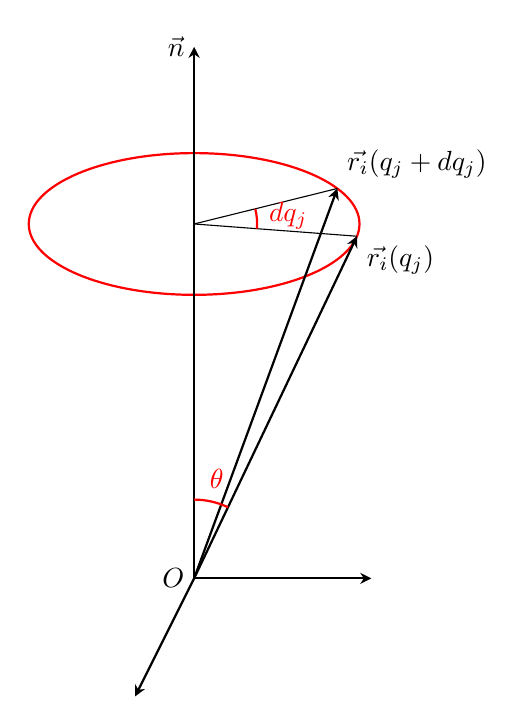
\begin{tikzpicture}[scale=1.5, 
  >={Stealth[length=4pt,width=4pt]},
  vector/.style={->,thick},
  charge/.style={circle,draw,fill=gray!20,minimum size=8pt,inner sep=0pt}
  ]
\def\R{1.4}
\def\r{0.6}
\def\thetaone{-10}
\def\thetatwo{30}
\coordinate (O) at (0,0);
\coordinate (A1) at (1.5,0);
\coordinate (A2) at (-0.5,-1);
\coordinate (N) at (0,4.5);
\coordinate (E) at (0,3);
\coordinate (P) at ($(E) + ({\R*cos(\thetaone)},{ \r*sin(\thetaone)})$);
\coordinate (Q) at ($(E) + ({\R*cos(\thetatwo)},{ \r*sin(\thetatwo)})$);
\draw (N) node[left] {$\vec{n}$};
\draw (O) node[left] {$O$};
\draw (P) node[below right] {$\vec{r_i}(q_j)$};
\draw (Q) node[above right] {$\vec{r_i}(q_j+dq_j)$};
% Ellipse
\draw[thick,red] (E) circle(\R cm and \r cm);
\draw[thick,->] (O)--(N);
\draw[thick,->] (O)--(P);
\draw[thick,->] (O)--(Q);
\draw[thick,->] (O)--(A1);
\draw[thick,->] (O)--(A2);
\draw[-] (E)--(P);
\draw[-] (E)--(Q);

% Angles
\pic[red,-,draw, thick,"$dq_j$",angle radius=8mm,angle eccentricity=1.5] {angle = P--E--Q};
% Angles
\pic[red,-,draw, thick,"$\theta$",angle radius=10mm,angle eccentricity=1.3] {angle = P--O--N};
%Points with rotation
\def\theta{0}
\coordinate (P) at ($(N) + ({2*cos(\theta)},{ sin(\theta)})$);
\def\theta{45}
\coordinate (Q) at ($(N) + ({2*cos(\theta)},{-sin(\theta)})$);
\end{tikzpicture}
\end{document}